\section{Durchführung}
\label{sec:Durchführung}
\subsection{Versuchsaufbau}

In \autoref{fig:aufbau} ist der schematische Aufbau der genutzten Messapparatur mit dem bereits beschriebenen Michelson-Interferometer dargestellt. 
\begin{figure}[H]
\centering
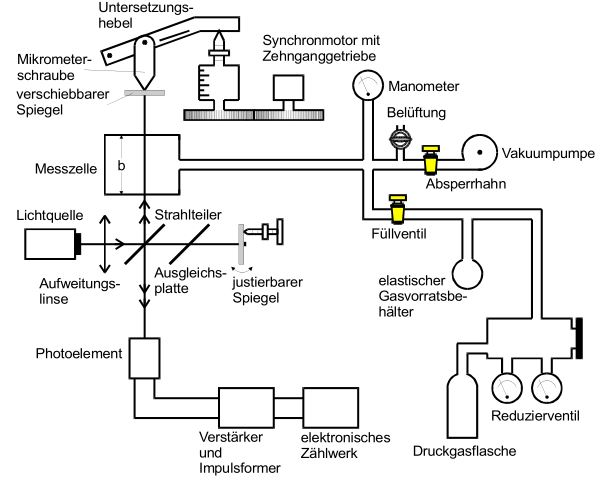
\includegraphics[width=\textwidth]{graphics/aufbau.JPG}
\caption{Schematischer Aufbau der genutzten Messapparatur \cite{anleitung}}
\label{fig:aufbau}
\end{figure}
\noindent
Die Länge der Messzelle $b$ beträgt dabei $b = \SI{50}{\milli\meter}$.
Die an den Geräten ablesbare Wellenlänge des genutzten Lasers beträgt $\SI{635}{\nano\meter}$ und die Hebelübersetzung am genutzten Motor beträgt $1:5,046$.
\subsection{Messvorgang}
Vor der eigentlichen Messung wird die Messapparatur kalibriert. Dabei werden die Spiegel so ausgerichtet, dass die einzelnen zu sehenden Lichtstreifen übereinander liegen. Als Hilfe wird bei der Justierung ein weißes Blatt Papier vor den Detektor gehalten, sodass die Lichtstreifen deutlicher zu sehen sind. Für die Messung wird dann der Motor angeschaltet und eine Wegstrecke von $5mm$ laufen gelassen, was an der Mikrometerschraube abgelesen wird. Dabei wird der Motor immer abwechselnd $5mm$ vor und zurück laufen gelassen und anschließend wird die vom Zählwerk gemessene Anzahl an Impulsen notiert. So werden insgesamt 8 Messreihen aufgenommen. \newline
\noindent
Bei der zweiten Messung wird der Motor nicht benötigt, sondern eine Druckänderung verursacht durch die Vakuumpumpe führt zu den gemessenen Impulsen.
Hier werden 16 Messwerte (8 mal aufgepumpt und 8 mal abgelassen) aus Druckänderung und gezählten Impulsen aufgenommen. Da die Vakuumpumpe per Hand bedient wird, muss bei der Versuchsdurchführung darauf geachtet werden, dass die Druckänderung nicht zu schnell geschieht damit die richtige Pulszahl gemessen wird. Die Druckänderung wird am Manometer der Vakuumpumpe abgelesen. Bei der Messung mit der Vakuumpumpe wurde die Messapparatur jeweils nach 8 und 12 aufgenommmenen Messwerten neu kalibriert, um bei der Impulszählung bestmögliche Ergebnisse zu erreichen. 

